\subsection{Dashboard principale}
La Dashboard principale costituisce il cruscotto di controllo primario del sistema, rappresentando una composizione di diversi pannelli che visualizzano i dati in tempo reale provenienti dai sensori.\\
\vspace{0.5cm}
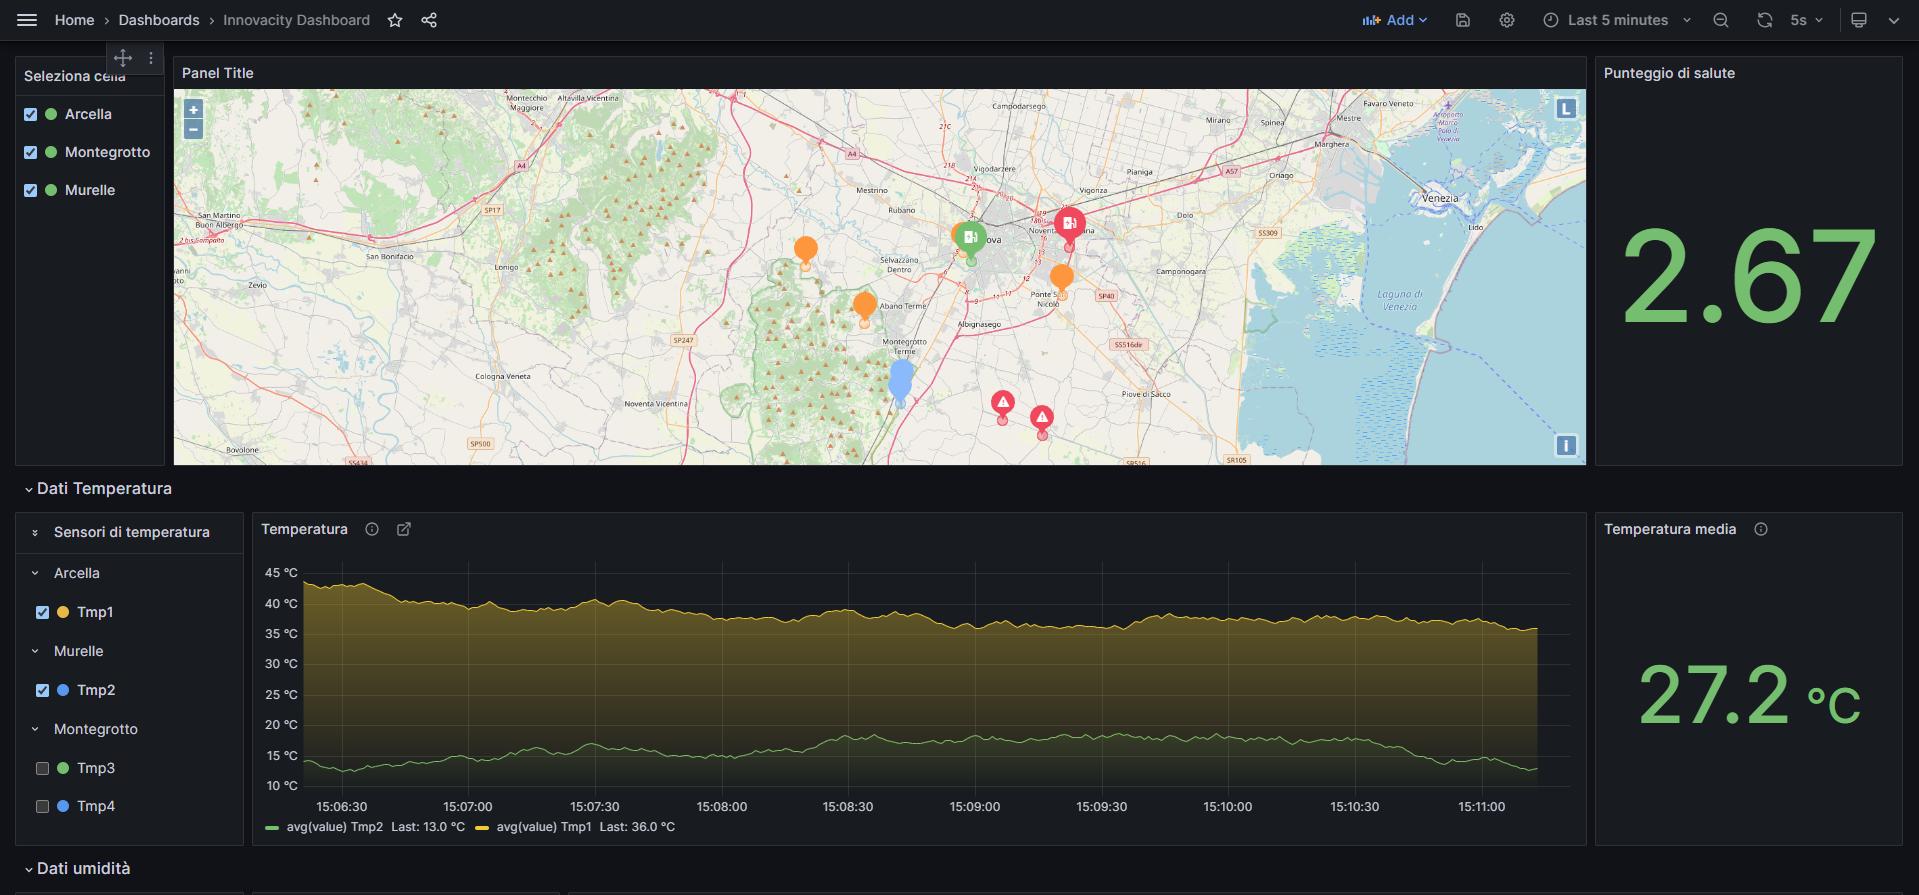
\includegraphics[width=16cm]{../Images/ManualeUtente/dashboard_principale.png}\\
\paragraph{Variabili di dashboard}
Prova\\
\vspace{0.5cm}
I pannelli sono strutturati in modo da essere suddivisi per categoria di dati al fine di facilitare la consultazione delle informazioni. Ciascun gruppo è opportunamente configurato per mostrare un tipo di dato specifico e per consentire interazioni mediante il cursore del mouse, fornendo dettagli aggiuntivi in risposta alle azioni dell'utente.\\ 
Cliccando su un bottone posto in ciascuno dei gruppi di pannelli, l'utente verrà reindirizzato in una dashboard contenente i dettagli relativi al gruppo selezionato.\\
\vspace{0.5cm}
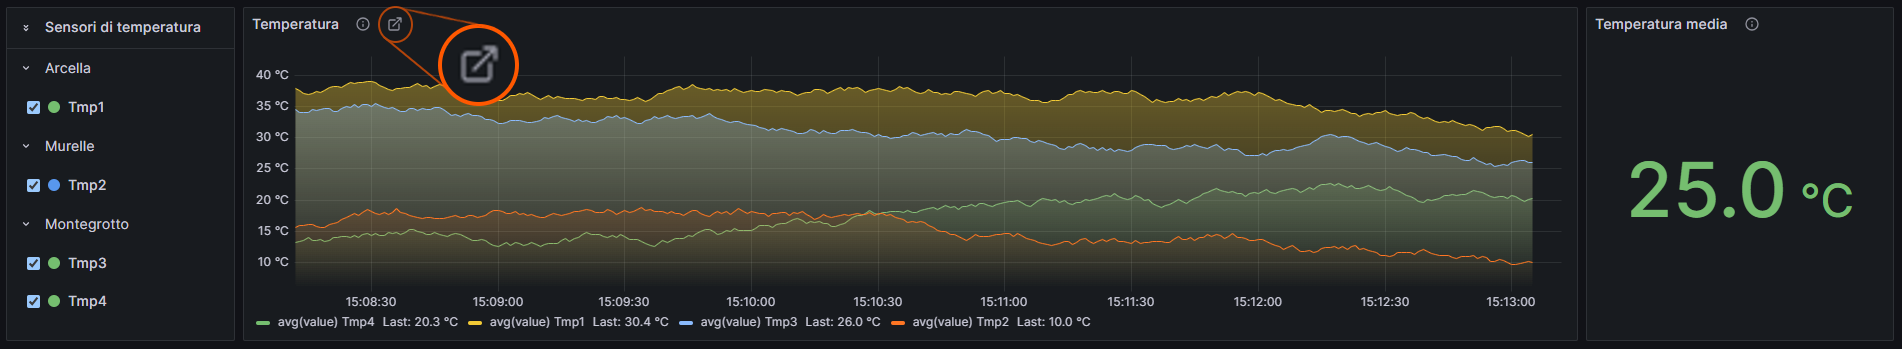
\includegraphics[width=16cm]{../Images/ManualeUtente/dettaglio_dashboard.png}

